% \special{dvipdfmx:config z 0}
\documentclass[UTF8,a4paper,AutoFakeBold,AutoFakeSlant]{article}
\usepackage[a4paper,left=2.8cm,right=2.6cm,top=3.7cm,bottom=3.5cm]{geometry}
\usepackage{CTEX}
% \usepackage{xeCJK}
\usepackage{graphicx}
\usepackage{pythonhighlight}
\usepackage[mathscr]{eucal}
\usepackage{mathrsfs}
\usepackage{booktabs}
\usepackage{capt-of} 
\usepackage{hyperref} 
\usepackage{abstract}
\usepackage{amsmath}
\usepackage{listings}
\usepackage{color}
\usepackage{caption}
\usepackage{subfigure}
\usepackage{enumerate}
\usepackage{amsfonts} 
\usepackage{CJK,CJKnumb}
\usepackage{float}
% \usepackage{gbt7714}
\usepackage{framed}
\usepackage{multirow}


\newcommand{\song}{\CJKfamily{song}}    % 宋体   (Windows自带simsun.ttf)
\newcommand{\fs}{\CJKfamily{fs}}        % 仿宋体 (Windows自带simfs.ttf)
\newcommand{\kai}{\CJKfamily{kai}}      % 楷体   (Windows自带simkai.ttf)
\newcommand{\hei}{\CJKfamily{hei}}      % 黑体   (Windows自带simhei.ttf)
\newcommand{\li}{\CJKfamily{li}}        % 隶书   (Windows自带simli.ttf) 
\newcommand{\ssong}{\CJKfamily{STSong}}

\xeCJKsetup{SlantFactor = 0.3}
% \xeCJKsetup{SlantFactor = -0.7}
\setCJKmainfont[BoldFont=simhei.ttf, SlantedFont=simkai.ttf]{simsun.ttc}



% -- 中文字体 --
%\setCJKmainfont{Microsoft YaHei}  % 微软雅黑
%\setCJKmainfont{YouYuan}  % 幼圆
%\setCJKmainfont{NSimSun}  % 新宋体
%\setCJKmainfont{KaiTi}    % 楷体
% \setCJKmainfont{SimSun}   % 宋体
%\setCJKmainfont{SimHei}   % 黑体
% \setCJKfamilyfont{hwsong}{STSong}
 
% -- 英文字体 --
% \setmainfont{Times New Roman}
% \setmainfont{DejaVu Sans}
% \setmainfont{Latin Modern Mono}
% \setmainfont{Consolas}
% \setmainfont{Courier New}


\usepackage{xcolor}  	%高亮使用的颜色
\definecolor{commentcolor}{RGB}{85,139,78}
\definecolor{stringcolor}{RGB}{206,145,108}
\definecolor{keywordcolor}{RGB}{34,34,250}
\definecolor{backcolor}{RGB}{220,220,220}

\usepackage{accsupp}	
\newcommand{\emptyaccsupp}[1]{\BeginAccSupp{ActualText={}}#1\EndAccSupp{}}

\usepackage{listings}
\lstset{						%高亮代码设置
	language=python, 					%Python语法高亮
	linewidth=0.95\linewidth,      		%列表list宽度
	%basicstyle=\ttfamily,				%tt无法显示空格
	commentstyle=\color{commentcolor},	%注释颜色
	keywordstyle=\color{keywordcolor},	%关键词颜色
	stringstyle=\color{stringcolor},	%字符串颜色
	%showspaces=true,					%显示空格
	numbers=left,						%行数显示在左侧
	numberstyle=\tiny\emptyaccsupp,		%行数数字格式
	numbersep=5pt,						%数字间隔
	frame=single,						%加框
	framerule=0.1pt,						%划线
	escapeinside=@@,					%逃逸标志
	emptylines=1,						%
	xleftmargin=3em,					%list左边距
	backgroundcolor=\color{backcolor},	%列表背景色
	tabsize=4,							%制表符长度为4个字符
	% gobble=4							%忽略每行代码前4个字符
}




\renewcommand{\abstractname}{}    % clear the title
\renewcommand{\absnamepos}{empty}
%去除摘要两边缩进
\makeatletter
  \renewenvironment{abstract}{%
      \if@twocolumn
        \subsection*{\abstractname}%
      \else
        \small
        \begin{center}%
          {\bfseries \abstractname\vspace{-.5em}\vspace{\z@}}%
        \end{center}%
      \fi}
      {}
  \makeatother
  \lstset{
    language=Matlab,
    keywords={break,case,catch,continue,else,elseif,end,for,function,
       global,if,otherwise,persistent,return,switch,try,while},
    basicstyle=\ttfamily,
    keywordstyle=\color{blue}\bfseries,
    commentstyle=\color{dkgreen},
    stringstyle=\color{dkpurple},
    backgroundcolor=\color{white},
    tabsize=4,
    showspaces=false,
    showstringspaces=false
 }

\title{\textbf{\textsf{{\textsf{LB2} \heiti{机器学习概论}}}}} 
\author{\ssong PB19151769~~~~~~马宇骁}
\date{}

% 去掉红框
\hypersetup{
colorlinks=true,
linkcolor=black
}

\begin{document}



\maketitle

\tableofcontents
\newpage



\section{实验要求}

完成类 `SVM1` 和 `SVM2` ,并且使用不同的算法去寻找支持向量机的解。 更具体地说,因为解决支持向量机的关键在于解决书本上的二次规划问题(6.6),你只需要使用两种不同的方法去解决(6.6)。剩下的部分,比如预测,内容可以相同。

在完成了类方法的部分之后,你需要测试你代码的效率。比较应当包含以下内容:

\begin{enumerate}
  \item 正确率,
  \item 计算(训练)的时间消耗。
\end{enumerate}

禁止使用 `` sklearn`` 或者其他的机器学习库,你只被允许使用 `numpy`, `pandas`, `matplotlib`, 和 \href{https://gitee.com/link?target=https%3A%2F%2Fdocs.python.org%2F3%2Flibrary%2Findex.html}{Standard Library}, 你需要从头开始编写这个项目。




\section{实验原理}

支持向量机(support vector machines, SVM)是一种二分类模型,它的基本模型是定义在特征空间上的间隔最大的线性分类器,间隔最大使它有别于感知机;SVM还包括核技巧,这使它成为实质上的非线性分类器。SVM的的学习策略就是间隔最大化,可形式化为一个求解凸二次规划的问题,也等价于正则化的合页损失函数的最小化问题。SVM的的学习算法就是求解凸二次规划的最优化算法。


\subsection{SVM算法原理}

SVM学习的基本想法是求解能够正确划分训练数据集并且几何间隔最大的分离超平面。即为分离超平面,对于线性可分的数据集来说,
这样的超平面有无穷多个(即感知机),但是几何间隔最大的分离超平面却是唯一的。

假设我们要寻找的最优分割平面:
\begin{equation*}
  \mathrm{w}^{*} \cdot \mathrm{x}+\mathrm{b}^{*}=0
\end{equation*}
把一个新的特征带入等号左边,如果大于0,说明为正类,小于0,说明为负类。

\subsection{SMO描述算法}

SVM的基本思路确定我们要优化的目标函数,即最大化几何间隔。在优化时我们取倒数,所以就是最小化目标函数。
通过拉格朗日乘数法来对目标函数进行优化,拉格朗日乘数法需要引入新的参数集 $\alpha$.
\begin{equation*}
  \mathrm{L}(\mathrm{w}, \mathrm{b}, \mathrm{a})=\frac{1}{2}\|\mathrm{w}\|^{2}-\sum_{\mathrm{i}=1}^{\mathrm{N}} \alpha_{\mathrm{i}} \mathrm{y}_{\mathrm{i}}\left(\mathrm{w} \cdot \mathrm{x}_{\mathrm{i}}+\mathrm{b}\right)+\sum_{\mathrm{i}=1}^{\mathrm{N}} \alpha_{\mathrm{i}}
\end{equation*}

原始问题:
\begin{equation*}
  \min _{\mathrm{w}, \mathrm{b}} \max _{\alpha} \mathrm{L}(\mathrm{w}, \mathrm{b}, \mathrm{a})
\end{equation*}

对偶问题,可以转换成拉格朗日对偶问题从而变成极大极小问题:
\begin{equation*}
  \max _{\alpha} \min _{\mathrm{w}, \mathrm{b}} \mathrm{L}(\mathrm{w}, \mathrm{b}, \mathrm{a})
\end{equation*}


\section{实验实现}

\subsection{算法流程}

\begin{enumerate}
  \item 初始化 $\alpha$参数集。数量等于example的数量。每个 $\alpha$与x 、y 对应;
  \item 选择两个 $\alpha$,分别记为$\alpha_1$ $\alpha_2$(第二个我用随机取);
  \item 使用$\alpha_1$,$\alpha_2$ 计算误差E1,E2;
  \begin{equation*}
    \begin{array}{c}
      \mathrm{g}(\mathrm{x})=\sum_{\mathrm{i}=1}^{\mathrm{N}} \alpha_{\mathrm{i}} \mathrm{y}_{\mathrm{i}} \mathrm{K}\left(\mathrm{x}_{\mathrm{i}}, \mathrm{x}\right)+\mathrm{b} \\
      \mathrm{E}_{\mathrm{i}}=\mathrm{g}\left(\mathrm{x}_{\mathrm{i}}\right)-\mathrm{y}_{\mathrm{i}}
      \end{array}
  \end{equation*}
  \item 计算范围,
  $\mathrm{y}_{1} !=\mathrm{y}_{2}$:
  \begin{equation*}
    \begin{array}{c}
      \mathrm{L}=\max \left(0, \alpha_{2}^{\text {old }}-\alpha_{1}^{\text {old }}\right) \\
      \mathrm{H}=\min \left(\mathrm{C}, \mathrm{C}+\alpha_{2}^{\text {old }}-\alpha_{1}^{\text {old }}\right)
      \end{array}
  \end{equation*}
  $\mathrm{y}_{1} ==\mathrm{y}_{2}$:
  \begin{equation*}
    \begin{array}{c}
      \mathrm{L}=\max \left(0, \alpha_{2}^{\text {old }}+\alpha_{1}^{\text {old }}-\mathrm{C}\right) \\
      \mathrm{H}=\min \left(\mathrm{C}, \alpha_{2}^{\text {old }}+\alpha_{1}^{\text {old }}\right)
      \end{array}
  \end{equation*}
  \item 计算$\eta$:
  \begin{equation*}
    \eta=\mathrm{K}_{11}+\mathrm{K}_{22}-2 \mathrm{~K}_{12}
  \end{equation*}
  \item 计算$\alpha_2^{new}$,并且限制在H,L区间内
  \begin{equation*}
    \begin{array}{c}
      \alpha_{2}^{\text {new }}=\alpha_{2}^{\text {old }}+\frac{\mathrm{y}_{2}\left(\mathrm{E}_{1}-\mathrm{E}_{2}\right)}{\eta} \\
      \alpha_{2}^{\text {new }}=\operatorname{clip}\left(\alpha_{2}^{\text {new }}, \mathrm{L}, \mathrm{H}\right)
      \end{array}
  \end{equation*}
  \begin{equation*}
    \alpha_{1}^{\text {new }}=\alpha_{1}^{\text {old }}+\mathrm{y}_{1} \mathrm{y}_{2}\left(\alpha_{2}^{\text {old }}-\alpha_{2}^{\text {new }}\right)
  \end{equation*}
  \item 对于b的更新:
  \begin{equation*}
    \begin{array}{c}
      \mathrm{b}_{1}^{\text {new }}=-\mathrm{E}_{1}-\mathrm{y}_{1} \mathrm{~K}_{11}\left(\alpha_{1}^{\text {new }}-\alpha_{1}^{\text {old }}\right)-\mathrm{y}_{2} \mathrm{~K}_{21}\left(\alpha_{2}^{\text {new }}-\alpha_{2}^{\text {old }}\right)+\mathrm{b}^{\text {old }} \\
      \mathrm{b}_{2}^{\text {new }}=-\mathrm{E}_{2}-\mathrm{y}_{1} \mathrm{~K}_{12}\left(\alpha_{1}^{\text {new }}-\alpha_{1}^{\text {old }}\right)-\mathrm{y}_{2} \mathrm{~K}_{22}\left(\alpha_{2}^{\text {new }}-\alpha_{2}^{\text {old }}\right)+\mathrm{b}^{\text {old }} \\
      \mathrm{b}=\left(\mathrm{b}_{1}^{\text {new }}+\mathrm{b}_{2}^{\text {new }}\right) / 2
      \end{array}
  \end{equation*}
  \item 转到第2步,直到收敛。
\end{enumerate}

最后训练好的参数预测时使用sign()函数。



\subsection{实验结果}

由于沿用了之前的数据集(5,100),样本较少,两种算法只是采用的核函数不同:线性与多项式(**2)。训练时间如下:
\begin{quotation}
  用时1.454028秒

  用时1.553001秒
\end{quotation}

训练曲线:
\begin{figure}[htbp]
  \centering
  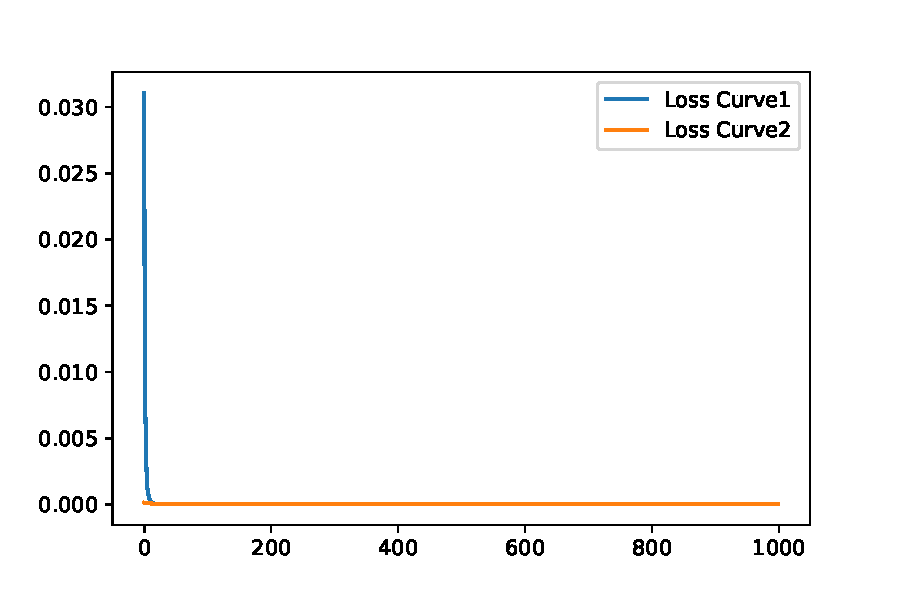
\includegraphics[scale=0.625]{loss.pdf}
  \caption{Loss Curve}
  \label{f1}
\end{figure}

训练预测准确率如下:
\begin{quotation}
  0.7721518987341772

  0.620253164556962
\end{quotation}



















% \bibliographystyle{gbt7714-numerical}
% % \bibliographystyle{7714-author-year}
% \bibliographystyle{ieeetr}
% \bibliography{bibl}

\end{document}